\todo{
\begin{itemize}
\item introduction
\item ``the blind way?'' - first attempts, visualisation directly with OCD
  \begin{itemize}
  \item Why it was bad idea
  \end{itemize}
\item Better approach - gantt chart
  \begin{itemize}
  \item Proposed first concept
  \item Time calculation via PERT (beta distribution)
  \item Gantt chart elements (progress bars, tree transaction view, transaction links,...)
  \end{itemize}
\end{itemize}}

The main goal of the thesis is to propose a concept of the mobile application which will be able to create the overview of critical business data and make decisions based on them. The concept is kept simple as possible and straightforward to achieve the goals. This chapter will describe each part of the concept and all conceptual features and functions. This chapter is divided to four parts:	
    \begin{enumerate}
      \item Which kind of data the application collects and how it works with them.
      \item What kind of overviews the application can display and how they are connected to the data.
      \item How real-time process visualization is done and how it communicates with internal business systems.
      \item And in the end, the concept of mobile application itself. The screens, supporting systems,\dots \todo{better}.
    \end{enumerate}
    
    \section{Business data}
    
    \subsection{Domain model}    
      \begin{figure}[ht!]
        \centering
        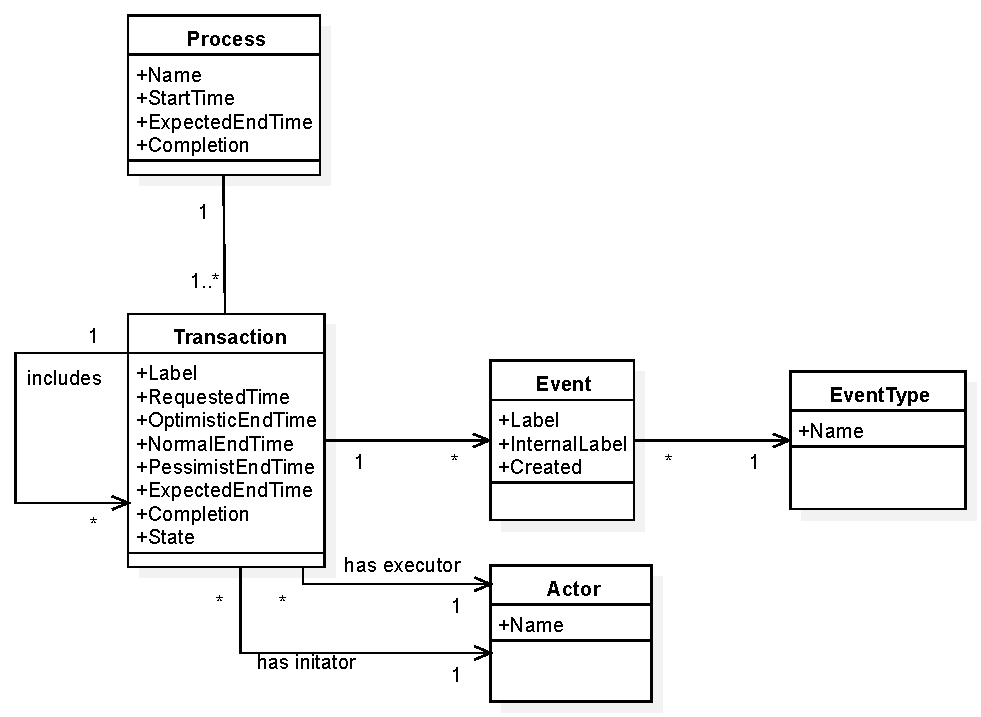
\includegraphics[width=12cm,keepaspectratio]{img/domain-core-model}
        \caption{Domain model \todo{change this image}}
        \label{fig:domain-core-model}
      \end{figure}    
      
      Figure \ref{fig:domain-core-model} shows domain model which describes how collected business data will be transformed for use in mobile application inside overviews and process visualization. 
    
    \section{Overviews}
    
    \section{Process visualization}
    
    \section{Mobile application concept}
	
	\todo{Domain model of collected data. Proposed way of real time visualization. Type of charts. Dashboard. Whole concept of application, e.g dashboard, editor. Functional specification, a.k.a example use cases?? Domain model of collected data.}
    
    \section{Analysis}    

   

	\section{The dashboard}
    Purpose of dashboard is provide centralized overview of processes such as average waiting time before process is completed or total amount of requests per day. The appearance of dashboard depends on user. \gls{dwma} provides customizable elements called widgets to achieve desired look for every user individually.

    \subsection{Widgets}  
     Widgets are small independent configurable components for displaying collected data from business processes. Each one has purpose. Notice that widgets are only user-friendly view of query above collected data. For editing widgets there is widget editor. User can simply edit properties of widget such as name, category, tags and of course source of data - the query and second important property is the type of widget. There are following types of widgets:
     
     \textbf{The summary widget} (\cref{fig:widget-summary}) provides, by it's name, chart with summarization of collected data. Concrete type of the chart depends on the user and on the data. Summary widget provides several types of charts:
     
     \begin{enumerate}
    	\item \textit{Pie} chart is used to illustrate numerical proportion.         
        \item  \textit{Bar} chart displays categorical data with numerical value.
        %\item \textit{Line}
    \end{enumerate}
      
      \begin{figure}[ht!]
          \centering
          
\includegraphics[width=6cm,keepaspectratio]{img/TODO-image}
          \caption{Summary widget example}
          \label{fig:widget-summary}
      \end{figure}   
    
   	Second type is \textbf{Time period} (\cref{fig:widget-time-period}). Time period displays data in some interval. Typically it can serve as overview \textit{``Number of requests for Rental payment per day"}.        
      
      \begin{figure}[ht!]
          \centering
          
\includegraphics[width=6cm,keepaspectratio]{img/TODO-image}
          \caption{Time period widget example}
          \label{fig:widget-time-period}
      \end{figure}
    
    Last type is \textbf{Single query} (\cref{fig:widget-single-query}) which allows display simple result from query. Prerequisite for query is that query returns one single record. 
      
      \begin{figure}[ht!]
          \centering
          
\includegraphics[width=6cm,keepaspectratio]{img/TODO-image}
          \caption{Single query example}
           \label{fig:widget-single-query}
      \end{figure}       
    
    \subsection{Query editor}
    
    \todo{Information about query editor}
    
    \begin{figure}[ht!]
          \centering
          
\includegraphics[width=6cm,keepaspectratio]{img/TODO-image}
          \caption{\todo{Query editor}}
      \end{figure}   
    
    \section{The real-time overview of process instance}
    \todo{Introduction about gantt chart. Make conversation about classic OCD / PSD diagrams and their pros and cons for visualizations}
    Provides the real-time overview of one concrete process instance.
On the left side is tree-view (like in folder explorer) of transactions. Each transaction has identifier and name.
On the top is the timeline which displays important events from the process. Above timeline is visualization itself. Each transaction is displayed as progress bar with some visual tweak, which will be discussed later.

	Each transaction can be at one of the following state, which has different visual: 
	\todo{Categories}
    
    \begin{description}
    	\item[Not active transaction] Is displayed as greyed out progress bar. It means that this instance of transaction will be probably started at some future time.

        \item[Active transaction] Progress bar is displayed with green colour to show current progress of instance transaction. 
        
        \item[Completed transaction] Progress bar is fulfilled with green colour. It means that given transaction successfully ended (was accepted).
        
        \item[Stopped transaction] Progress bar changed colour to red which indicates that transaction failed to complete due to fact that it was quitted or stopped. 
    \end{description}
    
 \subsection{Response and waiting links}
    \todo{Change this}
   Each transaction can have several child-transactions and also many conditional links. These conditions are displayed with arrows pointed to another transaction with the condition.
Conditions are divided into two categories.

If the condition is ``Some state of transaction A has to be done before transaction B can start (be requested)", e.g. transaction A must be stated before transaction B can be requested (\cref{fig:request-start-condition}).

\begin{figure}
  \centering
  
\includegraphics[width=6cm,keepaspectratio]{img/TODO-image}
  \caption{\todo{Request-start condition}}
  \label{fig:request-start-condition}
\end{figure}  

If condition is ``Some state of transaction A has to be done before transaction B can be at another state", e.g transaction A must be at least stated before transaction B can be promised (\cref{fig:state-state-condition}).

\begin{figure}
  \centering
  
\includegraphics[width=6cm,keepaspectratio]{img/TODO-image}
  \caption{\todo{State-state condition}}
  \label{fig:state-state-condition}
\end{figure}  

